\documentclass[a4paper, 11pt]{article}
\usepackage{comment} % enables the use of multi-line comments (\ifx \fi) 
\usepackage{lipsum} %This package just generates Lorem Ipsum filler text. 
\usepackage{fullpage} % changes the margin
\usepackage[brazilian]{babel}
\usepackage[utf8]{inputenc}
\usepackage[T1]{fontenc}
\usepackage{listings}
\usepackage{graphicx}

\begin{document}
%Header-Make sure you update this information!!!!
\noindent

\title{Reserva de Hoteis}

\maketitle

\section*{Descrição Geral}
Este é um sistema de busca de reserva mais barata em uma cadeia de hoteis. Dados a classe do cliente e as datas desejadas, é recomendado o hotel de menor custo e melhor qualidade. O sistema foi desenvolvido
utilizando a linguagem Python 2.7 e suas bibliotecas padrão.

\section*{Uso do Sistema}
Para rodar a aplicação, em um terminal partindo do diretório-raiz do projeto, executa-se o seguinte comando:

\begin{lstlisting}
python application.py <input_file>
\end{lstlisting}

Onde \emph{<input\_file>} é o arquivo com dados de entrada, um arquivo de texto onde cada linha é uma entrada seguindo o padrão da especificação do problema. Um arquivo de entrada
exemplo pode ser encontrado no diretório-raiz do projeto.

\begin{figure}[h]
  \begin{center}
   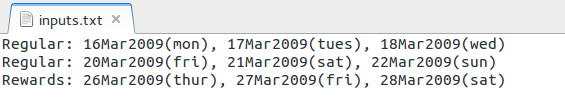
\includegraphics[scale=0.55]{images/input.png}
  \end{center}
  \caption{Arquivo de entrada exemplo}
\end{figure}

Para rodar a suite de testes, partindo-se do diretório-raiz deve-ser executar o comando:

\begin{lstlisting}
python -m unittest discover
\end{lstlisting}

\section*{Design do Sistema}
O núcleo do sistema é composto por 3 classes, cada qual representando uma entidade identificada no problema (cliente, hotel, cadeia de hoteis) e uma classe adicional responsável por gerenciar a leitura de dados de entrada.

\begin{figure}[h]
  \begin{center}
   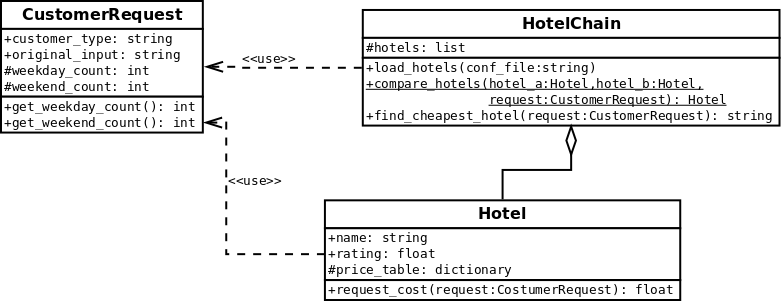
\includegraphics[scale=0.35]{images/core.png}
  \end{center}
  \caption{Diagrama simplificado apresentando as classes do núcleo do sistema}
\end{figure}

O sistema apresenta design flexível, orientado a arquivos de configuração. Deste modo é simples a adição de novos hoteis ou até mesmo novos tipos de clientes, bastando editar corretamente o arquivo de configuração config.xml localizado no diretório-raiz do projeto. Além disso, é definida uma interface comum para classes responsáveis pela leitura de entrada, facilitando a implementação de novos modos de fornecimento de dados ao programa (entrada de dados interativa, conexão de rede, etc).

\end{document}
